\section {Rastreamento}	

	O rastreamento de entidades, como pessoas ou objetos, é uma importante tarefa do campo da computação visual. A proliferação de computadores com um alto poder computacional, a disponibilidade de câmeras de alta qualidade a um preço acessível e a crescente necessidade de sistemas automáticos de análise de vídeos têm gerado um grande interesse em algoritmos de rastreamento~\cite{yilmaz}.

	% O rastreamento pode ser definido como o problema de estimar a trajetória de uma entidade em um plano de imagem a medida em que se move na cena. Em outras palavras, um rastreador atribui rótulos as entidades monitoradas em diferentes quadros de um vídeo~\cite{yilmaz}.

	A detecção e o rastreamento de pessoas tem um grande potencial em aplicações em domínios tão diversos como animação, interação humano-computador, vigilância automatizada (monitorar uma cena para detectar atividades suspeitas), entre outros~\cite{yilmaz}. Por esta razão, tem havido um crescimento notável na investigação deste problema.

	O rastreamento de pessoas em um ambiente é considerada como uma tarefa complexa devido a:

		\begin{enumerate}
			\item complexidade do corpo humano;
			\item alta dinamicidade do ambiente;
			\item ruído nas imagens~\cite{yilmaz};
			\item complexidade do movimento das pessoas;
			\item oclusões parciais ou totais de pessoas;
			\item variação na iluminação do ambiente~\cite{yilmaz};
			\item processamento em tempo-real~\cite{yilmaz};
		\end{enumerate}

	Algumas dessas dificuldades podem ser vencidas com a utilização de imagens de profundidade ao invés de imagens de cor ou intensidade. As imagens de profundidade, além de serem muito pouco sensíveis as variações de iluminação, provêem um fácil entendimento da estrutura da cena, que pode ser utilizada para simplificar as tarefas de rastreamento. Além disso, as câmeras que obtêm imagens de profundidade estão comercialmente disponíveis a um preço acessível~\cite{nikos}.

	Várias abordagens para rastreamento de objetos já foram propostas. Basicamente, elas se diferem na forma que tratam as seguintes perguntas~\cite{yilmaz}: 
		
		\begin{itemize}
			\item Qual representação do objeto é adequada para o rastreamento~\cite{yilmaz}?
			\item Quais características na imagem devem ser utilizadas~\cite{yilmaz}?
			\item Como o movimento, aparência e a forma do objeto deve ser modelada~\cite{yilmaz}? 
		\end{itemize}

	As respostas para estas perguntas dependem do contexto/ambiente onde o rastreamento será utilizado e do uso final das informações de rastreamento~\cite{yilmaz}.

	O rastreamento de pessoas geralmente inicia com o processo de segmentação da
	imagem da pessoa do resto da imagem. Depois, essas imagens segmentadas são
	transformadas em outras representações para reduzir a quantidade de informação
	ou para atender a um determinado algoritmo. Com isso, deve-se definir como as
	pessoas vão ser rastreadas quadro a quadro~\cite{moeslund}.

	Basicamente, o processo de rastreamento pode ser dividido em duas etapas:

		\begin{enumerate}
			\item Detecção do objeto;
			\item Rastreamento do objeto detectado;
		\end{enumerate}

	Antes de falar mais sobre cada uma dessas etapas e os métodos existentes para cada, será apresentado as maneiras existentes de representar as entidades rastreadas e sobre as características presentes nas imagens que podem ser utilizadas.

%%%%%%%%%%%%%%%%%%%%%%%%%%%%%%%%%%%%%%%%%%%%%%%%%%%%%%%%%%%%%%%%%%%%%%%%%%%%%%%%%%%%%%%%%%%%%%%%%%%%%%%%%%%%%%%

\subsection{Representação da Entidade}
\label{sec:representacao-objeto}

	Nos sistemas de rastreamento, as entidades rastreadas devem ser representadas de alguma maneira. Geralmente, as representações são baseados em suas formas, existindo uma forte relação entre a representação e o algoritmo de rastreamento escolhido~\cite{yilmaz}. A representação é escolhida baseada no domínio da aplicação e as mais utilizadas são:

	\begin{figure}[hbt]
		\begin{center}
			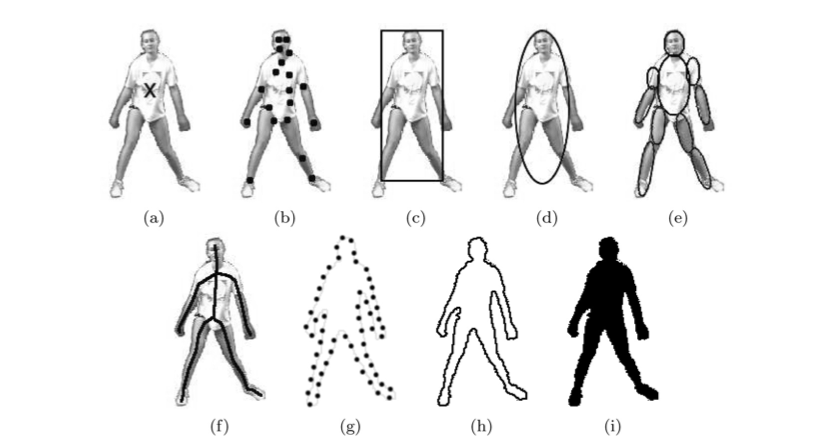
\includegraphics[scale=0.5]{figuras/2.FundamentacaoTeorica/representacao.png}
		\end{center}
		\caption{Representações de entidades rastreadas. (a) Centróide, (b) múltiplos pontos, (c) representação retangular, (d) representação elíptica, (e) representação de múltiplas partes, (f) esqueleto, (g) contorno por pontos,(h) contorno completo, (i) silhueta~\cite{yilmaz}}
		\label{representacao}
	\end{figure}

	\begin{itemize}
		\item \textbf{Pontos:} a entidade é representada por um ponto, como por exemplo a centróide~\cite{veenman} da Figura \ref{representacao}(a), ou por vários pontos~\cite{serby}, como por exemplo na Figura \ref{representacao}(b). Essa representação é mais adequada para rastreamento de entidades que ocupam uma pequena região na imagem~\cite{yilmaz};

		\item \textbf{Formas geométricas primitivas:} a entidade é representada por formas geométricas simples como um retângulo ou uma elipse, como mostrados nas Figuras \ref{representacao}(c) e (d)~\cite{comaniciu}. Essa representação é mais adequada para simples entidades rígidas~\cite{yilmaz};

		\item \textbf{Silhueta e Contorno:} representação por contorno define os limites de uma entidade, como mostrado nas Figuras \ref{representacao}(g) e (h). A região interna do contorno é chamada de Silhueta, como mostrado na Figura \ref{representacao}(i). Essa representação é mais adequada para rastrear entidades complexas de forma não rígida~\cite{yilmaz, yilmaz2}. Ela é popular devido a sua simplicidade. A silhueta ou contorno de uma entidade pode ser obtida definindo métodos de limiarização ou subtração, podendo ser utilizada tanto com imagens 2D quanto 3D. A representação 2D geralmente é mais simples~\cite{moeslund};

		\item \textbf{Modelos de formas articuladas:} entidades articuladas são compostos por partes do corpo que se ligam por meio de juntas. Para representá-las, utiliza-se figuras geométricas para cada parte do corpo, como mostrado na Figura \ref{representacao}(e)~\cite{yilmaz};

		\item \textbf{Modelos de esqueletos:} modelos de esqueletos são extraídos da entidade rastreada, como mostrado na Figura \ref{representacao}(f). Essa representação pode ser utilizada tanto para entidades articuladas rígidas quanto não rígidas~\cite{yilmaz};
	\end{itemize}

	Para rastreamento de pessoas a representação por meio de contorno ou silhuetas são as mais adequadas~\cite{yilmaz}.

	O rastreamento de várias pessoas de maneira simultânea é considerada uma tarefa muito complexa. As representações das pessoas rastreadas podem se dividir ou fundir em novas representações devido a possíveis oclusões ou ruídos na imagem, e a aparência do objeto pode variar devido a sombras e mudanças da iluminação~\cite{moeslund}.

%%%%%%%%%%%%%%%%%%%%%%%%%%%%%%%%%%%%%%%%%%%%%%%%%%%%%%%%%%%%%%%%%%%%%%%%%%%%%%%%%%%%%%%%%%%%%%%%%%%%%%%%%%%%%%%

\subsection{Seleção de características para rastreamento}

	A seleção das características é uma tarefa crítica para o rastreamento e está fortemente relacionada com a representação da entidade. Em geral, a seleção procura as características mais singulares para que a entidade rastreada seja facilmente distinguida~\cite{yilmaz}. As características mais comuns utilizadas atualmente são:

	\begin{itemize}
		\item \textbf{Cor:} a cor da entidade é influenciada principalmente por duas
		características: a distribuição da iluminação e a propriedade de reflectância da
		entidade. Geralmente, a representação \textit{RGB} é utilizada para representar
		a cor~\cite{yilmaz};

		\item \textbf{Borda:} os limites de uma entidade geram uma grande variação de
		intensidade na imagem e são menos sensíveis a variações na iluminação comparado
		com as cores. A detecção por meio das bordas é utilizada para identificar essas
		variações de intensidade na imagem. Os algoritmos que detectam as bordas
		geralmente as utilizam para representação dos mesmos~\cite{yilmaz};

		\item \textbf{Fluxo óptico:} é um campo denso de vetores de deslocamento que
		define a tradução de cada \textit{pixel} em uma região. Ele é calculado a
		partir da restrição de luminosidade, que pressupõe a constância de brilho nos
		\textit{pixels} correspondentes nos quadros consecutivos~\cite{yilmaz,
		horn};

		\item \textbf{Textura:} é a medida da intensidade da variação da superfície que
		quantifica propriedades como suavidade e regularidade. A Textura é menos
		sensível a variação da iluminação comparado com a cor~\cite{yilmaz};

	\end{itemize}

De todas as características, a mais utilizada para rastreamento é a cor~\cite{yilmaz}.

%%%%%%%%%%%%%%%%%%%%%%%%%%%%%%%%%%%%%%%%%%%%%%%%%%%%%%%%%%%%%%%%%%%%%%%%%%%%%%%%%%%%%%%%%%%%%%%%%%%%%%%%%%%%%%%

\subsection{Detecção de entidades}
\label{sec:deteccao-objeto}

	Todo método de rastreamento requer um mecanismo de detecção de entidades que
	pode ser realizada a cada quadro obtido ou na primeira vez que a
	entidade aparece no vídeo. Os método mais populares são:


	\begin{itemize}
		\item \textbf{Detector de pontos:} esses detectores são usados para encontrar
		pontos de interesses dentro da imagem que tem uma expressiva textura na sua
		respectiva localização. Pontos de interesse são amplamente usados no contexto do
		movimento e no rastreamento. A qualidade desejável para o ponto de interesse é
		que seja invariante diante das mudanças de iluminação e ângulo de visão da
		câmera~\cite{yilmaz}.
			
		\item \textbf{Subtração de fundo:} é um método popular para segmentação de
		movimento, especialmente nas situações em que o plano de fundo é relativamente
		estático. Ele detecta as regiões de movimento na imagem obtendo a diferença
		\textit{pixel} a \textit{pixel} entre o quadro corrente e o
		quadro referente ao plano de fundo~\cite{weiming}. Geralmente, um
		algoritmo de componentes conectadas é aplicado para obter regiões conectadas que
		correspondem a uma entidade~\cite{yilmaz}.
		
		\item \textbf{Segmentação:} o objetivo do algoritmo de segmentação é particionar
		a imagem em regiões com certo grau de similaridade. Todo algoritmo de
		segmentação tem dois problemas: o critério para definir uma boa partição e o
		método para arquivar particionamentos eficientes~\cite{yilmaz, shi}.

		\item \textbf{Aprendizagem supervisionada:} a detecção de entidades pode ser
		feita pelo aprendizado automático de diferentes entidades de um conjunto de
		exemplos por meio de um mecanismo de aprendizado. Esse aprendizado requer o
		armazenamento de um um conjunto de \textit{templates}. A partir desse conjunto
		de informações, o algoritmo gera uma função que mapeia as possíveis entradas
		para as saídas desejadas. Um problema padrão é a classificação onde a função
		gera um valor contínuo a partir de um determinado comportamento da entidade. No
		contexto da detecção de entidades as informações armazenadas são compostas por
		um par de características de entidades e uma classe associada onde ambos os
		valores são manualmente definidos. A seleção de características tem um papel
		importante no desempenho da classificação, portanto, é importante usar um
		conjunto de características que seja possível discriminar uma classe das
		outras~\cite{yilmaz}.
	\end{itemize}

%%%%%%%%%%%%%%%%%%%%%%%%%%%%%%%%%%%%%%%%%%%%%%%%%%%%%%%%%%%%%%%%%%%%%%%%%%%%%%%%%%%%%%%%%%%%%%%%%%%%%%%%%%%%%%%

\subsection{Rastreamento de entidades}
\label{sec:rastreamento}

	O objetivo do rastreamento de entidades é conhecer a trajetória do mesmo no
	tempo localizando sua posição em cada quadro. O rastreamento também pode
	prover a região completa na imagem ocupada pela entidade a cada
	instante~\cite{yilmaz}.

	As atividades de detecção de entidades e de estabelecimento de correspondências
	entre elas e as instâncias dos quadros podem ser realizadas tanto
	separadamente como concomitantemente. No primeiro caso, as prováveis regiões de
	entidades são obtidas e o rastreador encontra correspondência entre as entidades
	e os quadros. No último caso, as prováveis regiões e as correspondências
	são feitas juntas e estimadas pela atualização iterativa da localização da
	entidade e de regiões de informações obtidas dos quadros
	anteriores~\cite{yilmaz}.\

	Os métodos de rastreamento de entidades mais utilizados atualmente são:

	\begin{itemize}
		\item \textbf{Rastreamento de pontos:} as entidades detectadas a cada quadro
		são representadas por pontos e a associação entre os pontos é feita com base no
		estado anterior da entidade que pode incluir a posição e o movimento. Essa
		abordagem requer um mecanismo externo para detectar a entidade a cada
		quadro~\cite{yilmaz};
		
		\item \textbf{Rastreamento de núcleo}: as entidades são rastreados pelo cálculo
		do movimento do núcleo em quadros consecutivos. Esse movimento
		geralmente esta na forma de transformações paramétricas como translação e
		rotação. O núcleo se refere ao formato ou aparência da entidade~\cite{yilmaz}.
		
		\item \textbf{Rastreamento de silhuetas:} o rastreamento é feito estimando a
		região da entidade a cada quadro. Esse método utiliza informações contidas
		dentro da região estimada. Esta informação pode ser na forma de densidade de
		aparência e modelos de forma que estão, geralmente, na forma de mapas de borda.
		Dado os modelos de entidades, silhuetas são rastreadas por qualquer forma de
		correspondência ou evolução de contorno. Ambos os métodos podem ser
		essencialmente considerados como segmentação de entidades aplicada no domínio
		temporal utilizando os priores gerados a partir dos quadros
		anteriores~\cite{yilmaz}.
	\end{itemize}

Com as entidades rastreadas, para obter a posição dos mesmos deve-se obter
informações de profundidade. Na próxima seção falaremos sobre como essas
informações são obtidas utilizando imagens de profundidade.




